\documentclass[10pt, dvipsnames]{beamer}
%\setbeameroption{show only notes}

\usetheme[width = 3\baselineskip]{Berkeley}
\usecolortheme{seahorse}

% keine Navgationssymbole
%\setbeamertemplate{navigation symbols}{}

% Navigationssymbole durch Foliennummer ersetzen
\setbeamertemplate{page number in head/foot}[totalframenumber]
\setbeamertemplate{navigation symbols}{\footnotesize\usebeamertemplate{page number in head/foot}}

% Hervorhebung des derzeitigen Abschnitts in Rot

\makeatletter

\setbeamertemplate{subsection in sidebar}
{%
    \beamer@sidebarformat{5pt}{subsection in sidebar}{\color{red!80!gray}\tiny\insertsubsectionhead}% color and font size subsection << <<
}

\setbeamertemplate{subsection in sidebar shaded}
{%
    \beamer@sidebarformat{5pt}{subsection in sidebar shaded}{\color{black!60}\tiny\insertsubsectionhead}%  color and fontsize <<<
}

\setbeamertemplate{section in sidebar}% color and font size section << <<<
{%
\vbox{%
%       \vskip1ex% <<<<
    \beamer@sidebarformat{3pt}{section in sidebar}{\color{red!80!gray}\tiny\insertsectionhead}%
}%
}

\setbeamertemplate{section in sidebar shaded}% color and font size section << <<<
{%
\vbox{%
%       \vskip1ex% <<<<
    \beamer@sidebarformat{3pt}{section in sidebar shaded}{\color{black!60}\tiny \insertsectionhead}%
}%
}

\makeatother

\AtBeginSection[]
{
  \begin{frame}
    \frametitle{Outline}
    \tableofcontents[currentsection,currentsubsection]
  \end{frame}
}

% Titelfolie

\title[Lotka-Volterra Models]{Mathematical Analysis\\ and Numerical Simulations\\ of\\General Lotka-Volterra Systems}
 



\author[Graß Tobias Simon]{Graß Tobias Simon}
\date{January 11, 2023}
\institute[University Vienna]{University of Vienna}
\logo{
\includegraphics[scale=0.1]{Grafiken/logo_univie.jpg}}


% Pakete 

% Rechtschreibung % Layout % Literatur
\usepackage[T1]{fontenc}
\usepackage{lmodern}
\usepackage[english]{babel}
\usepackage[utf8]{inputenc}
\usepackage{csquotes}
\usepackage[font=scriptsize]{caption}
\usepackage[natbib,abbreviate=true,doi=false,style=numeric-comp,giveninits=true,sorting=none]{biblatex}
	\addbibresource{MyBibliography.bib}
\renewcommand*{\bibfont}{\tiny}


% Grafiken & Animationen
\usepackage{graphicx}
\usepackage{xcolor}
\usepackage{tikz}
\usepackage{animate}
\usepackage{pgfplots}
\usepackage{pdfpcnotes}
\usetikzlibrary{arrows.meta,backgrounds}
\usepgfplotslibrary{fillbetween}


% Mathematik 
\usepackage{amssymb}
\usepackage{amsmath}
\usepackage{amsfonts}
\usepackage{amsthm}
\usepackage{physics}
\usepackage{nicematrix}
\NiceMatrixOptions{
code-for-first-row = \color{blue!50} ,
code-for-first-col = \color{blue!50} ,
}

\newtheorem*{remark}{Remark}
\newtheorem{theo}{Teorema}
\AtBeginEnvironment{theo}{%
  \setbeamercolor{block title}{use=example text,fg=black,bg=yellow!75!black}
  \setbeamercolor{block body}{parent=normal text,use=block title example,bg=yellow!10}
}

\newcommand*\laplace{\mathop{}\!\mathbin\bigtriangleup}

\setcounter{biburllcpenalty}{9000}% Kleinbuchstaben
\setcounter{biburlucpenalty}{9000}% Großbuchstaben

\begin{document}
\begin{frame}
\pnote{Greeting}
\pnote{Introduction}

\titlepage
\end{frame}

\section[Example]{Introductory Example}

\begin{frame}{Hare and Lynx Population Dynamics}
\pnote{Species: Canadian Lynx & Snowshoe Hare}
\pnote{Hudson Bay Company: Pelt Trading}
\pnote{Lynx mainly eat hare about 2 every three days (abundance)}
\pnote{Hare population stays between 1k - 70k}
\pnote{Lynx population stays between 3k - 60k}
\pnote{Phase shift}

\begin{figure}
    \centering
    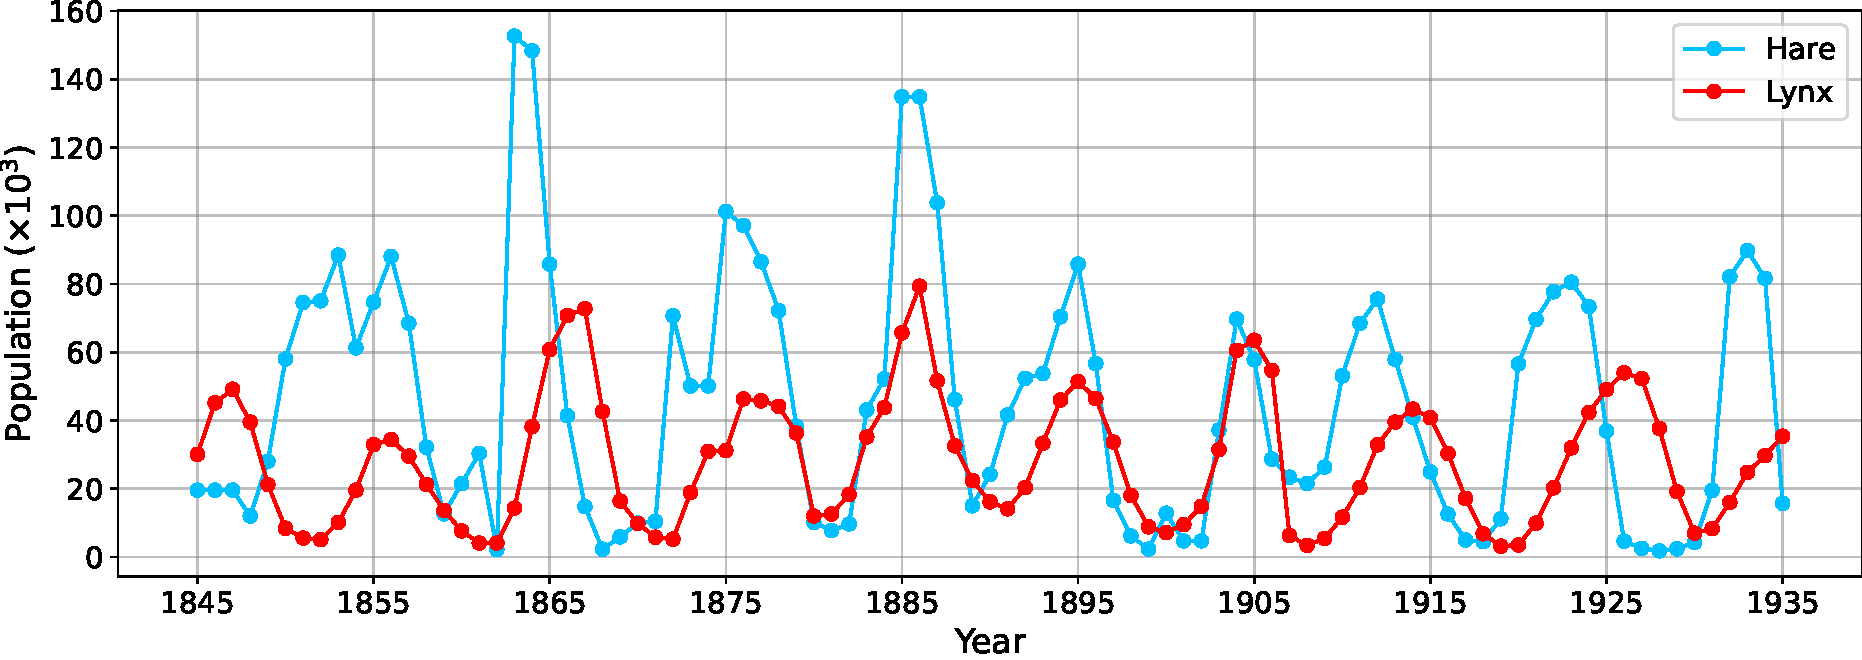
\includegraphics[width = \linewidth]{Grafiken/intro_example.pdf}
    \caption{Development of the population sizes of lynx and hares in the northern boreal forests of North America.}
    \label{fig:intial_example}
\end{figure}

\end{frame}
\section[General System]{The General Lotka-Volterra Equations}
\begin{frame}{General Lotka-Volterra Equations}
\pnote{Intrinsic growth/decay rate: $r_i$}
\pnote{Interaction coefficients: $a_{ij}$}
\pnote{Three cases: mutualistic, competitive, predator-prey dynamics}
\pnote{Immigration is not possible in this system since if $x(0)>0 \implies x(t)>0$ for all $t$}
\pnote{Simple: No intraspecific interaction between members of the same population}

\begin{definition}[General Lotka-Volterra Equations]
    The general Lotka-Volterra equations for a $n$-species model is the system
    \begin{align}\label{eq:general_lotka_volterra_equations}
        F_i(x) = \frac{\mathrm{d}x_i}{\mathrm{d}t} = x_i \left(r_i + \sum_{j = 1}^{n}a_{ij} x_j \right)
    \end{align}
    with $i = 1, 2, \ldots, n$. The matrix $A = (a_{ij})_{i, j = 1, 2, \ldots, n}$ is called the interaction matrix of the system. The vector $\vectorbold{r} = (r_1, r_2, \ldots, r_n)$ contains the growth rates of the $i$-th species \cite[12, 64 \psq]{10.25365/thesis.45530, Volterra1931}.
\end{definition}\pause

\begin{remark}
    \begin{itemize}
        \item The state space of system (\ref{eq:general_lotka_volterra_equations}) is the nonnegative orthant $\mathbb{R}^n$.
        \item If $a_{ii} = 0$ for all $i = 1, 2, \ldots, n$ the system is called simple.
    \end{itemize}
\end{remark}
    
\end{frame}
\subsection[Simplified System]{Simple Predator-Prey Model for $n=2$}
\begin{frame}{2-Species Predator-Prey Model}
\pnote{Alfred James Lotka (1880 - 1949)}
\pnote{Vito Volterra (1860 - 1940)}
\pnote{Both studied pred-prey interactions during 1920-1926; conclusion: periodic oscillation}
\pnote{Volterra: $n$-species model with respect to the past (delay kernels)}
\pnote{$x_1$ prey}
\pnote{$x_2$: predator}

\begin{definition}[2-dimensional Predator-Prey Model]
    The system of equations
    \begin{align}\label{eq:2d_simple_model}
    \begin{split}
        \frac{\mathrm{d}x_1}{\mathrm{d}t} &= x_1 (r_1 - a_{12}x_2) \\
        \frac{\mathrm{d}x_2}{\mathrm{d}t} &= x_2 (-r_2 + a_{21}x_2)
    \end{split}
    \end{align}
    for $r_1, r_2, a_{12}, a_{21} > 0$ is called simple predator-prey model and is a special case of system (\ref{eq:general_lotka_volterra_equations}).
\end{definition}

\end{frame}

\begin{frame}{Implications for the Ecosystem}

\begin{itemize}
    \item The prey population $x_1$ has an unlimited food supply.\pause
    \item The growth of $x_1$ is exponential in the absence of their predators $x_2$, i.e. $\frac{\mathrm{d}x_1}{\mathrm{d}t} = r_1 x_1$.\pause
    \item For $x_1 = 0$, the decay of $x_2$ is also exponential, i.e. $\frac{\mathrm{d}x_2}{\mathrm{d}t} = -r_2 x_1$ \cite[4 \psq]{predatorpreymodel}.\pause
    \item The biotope is completely isolated from external influences \cite[199]{theoryvsempiry}.
\end{itemize}
    
\end{frame}
\subsubsection{Simulations}
\begin{frame}{Numerical Results}
\pnote{Periodicity}
\pnote{Phase shift}

\begin{figure}
    \centering
    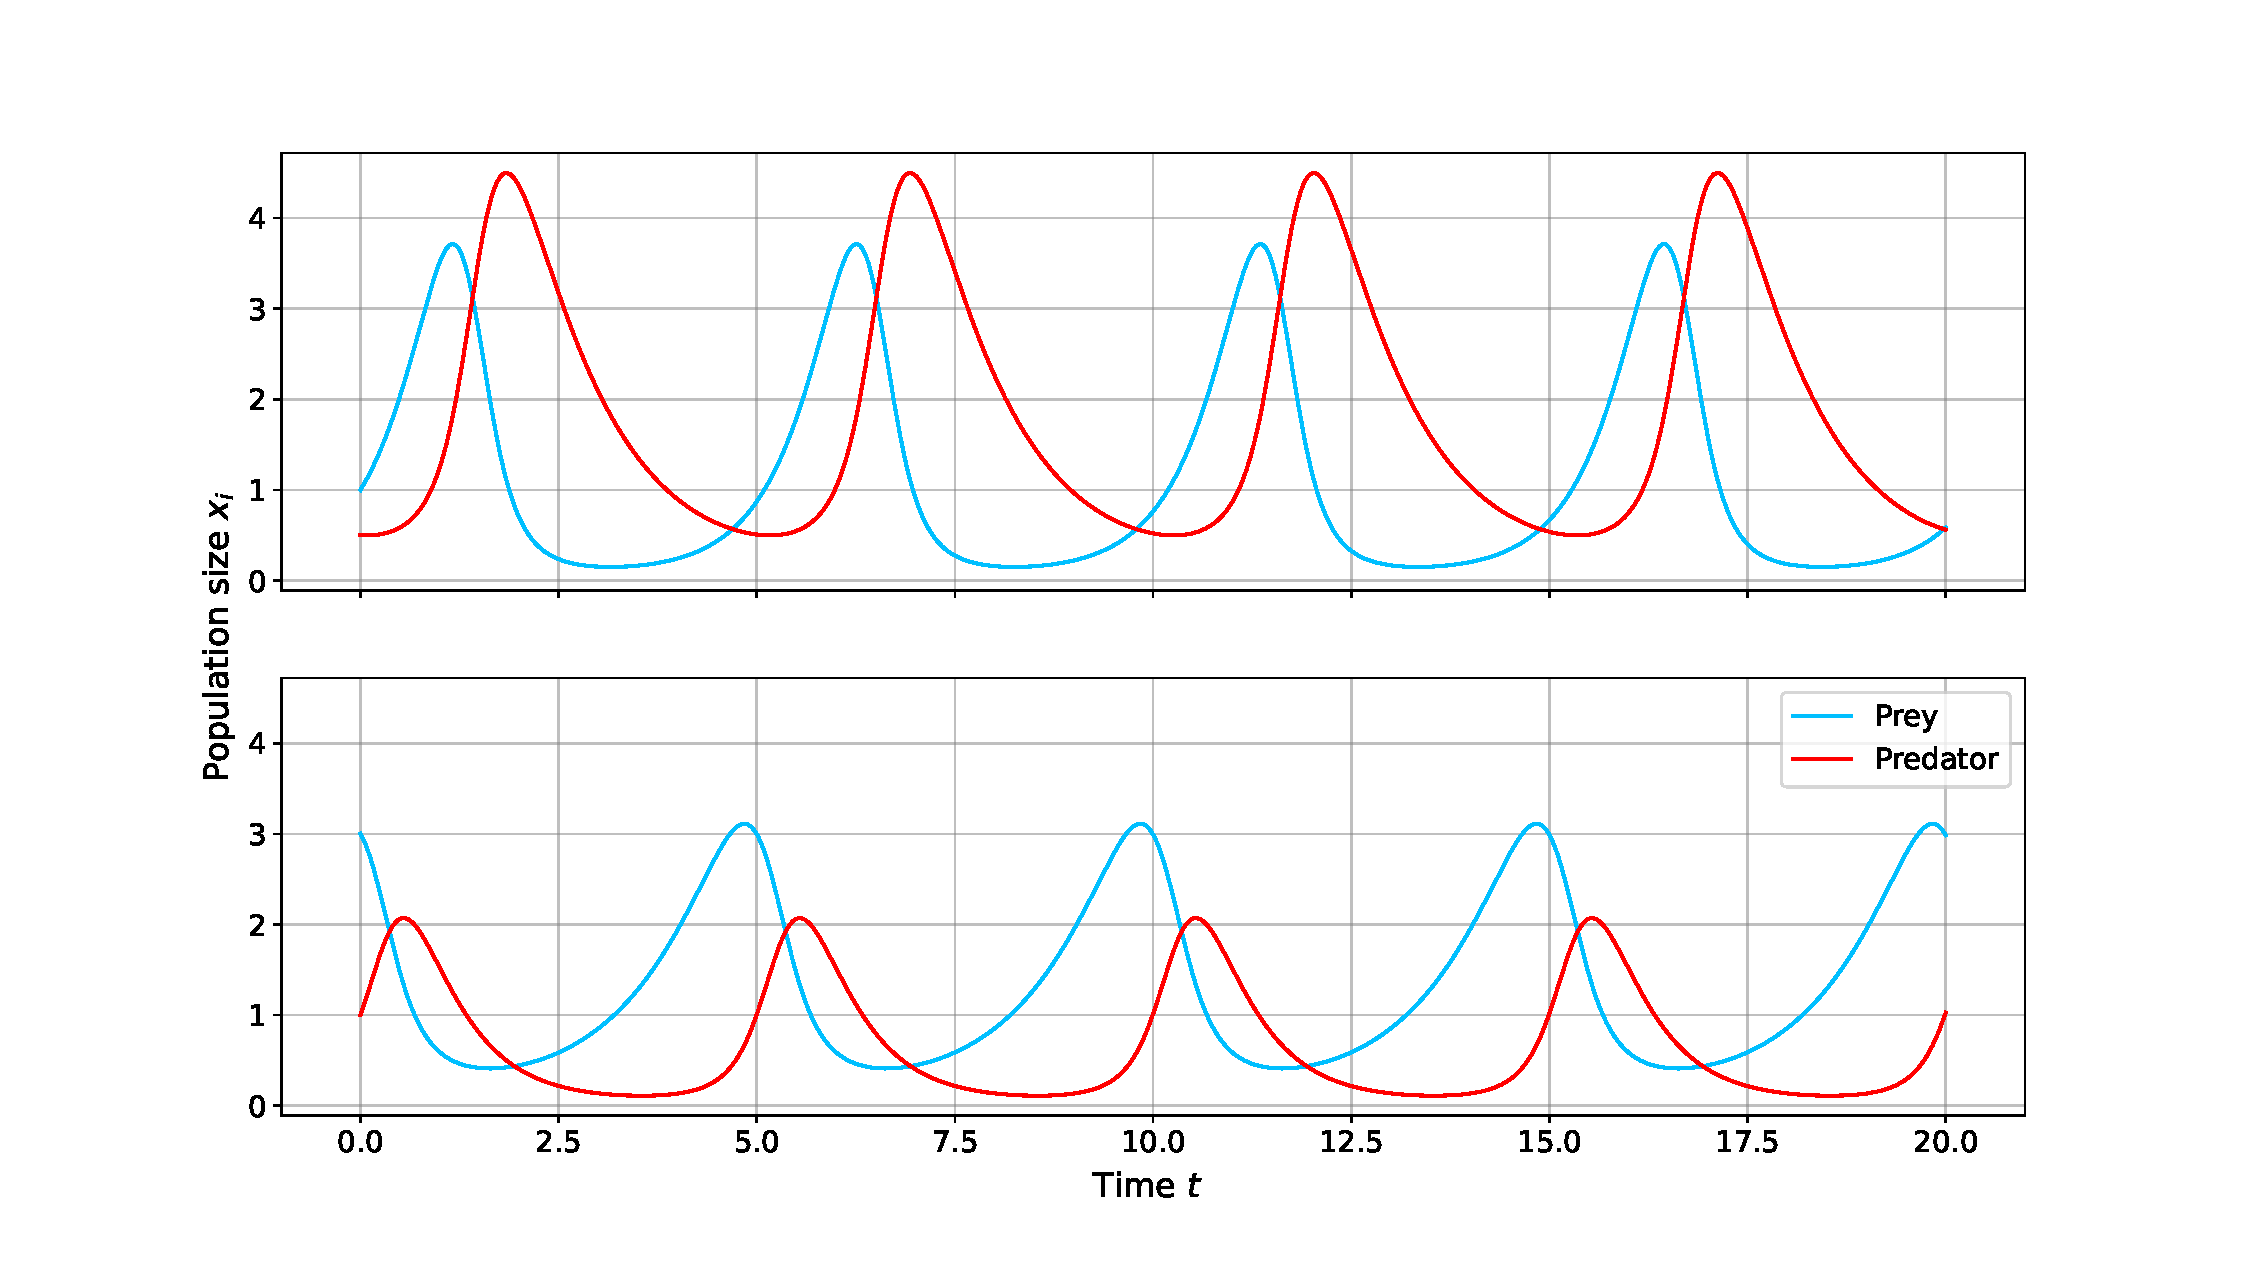
\includegraphics[width = \linewidth]{Grafiken/solution_2d_simple_model.pdf}
    \caption{Numerical solutions of the 2-species predator-prey model (\ref{eq:2d_simple_model}) introduced by Lotka and Volterra. The first system was solved for the initial condition $x_1(0)= 1, x_2(0)=0.5$, the second set of equations for $x_1(0)= 3, x_2(0)=1$ respectively.}
    \label{fig:numerical_solutions_2d_simple_model}
\end{figure}
    
\end{frame}
\begin{frame}{Slope Field and Phase Space Representation}
\pnote{Vectors are normalized (same length)}
\pnote{Periodicity: closed trajectory around stable center $\Bar{s}_1$}

    \begin{figure}
        \centering
        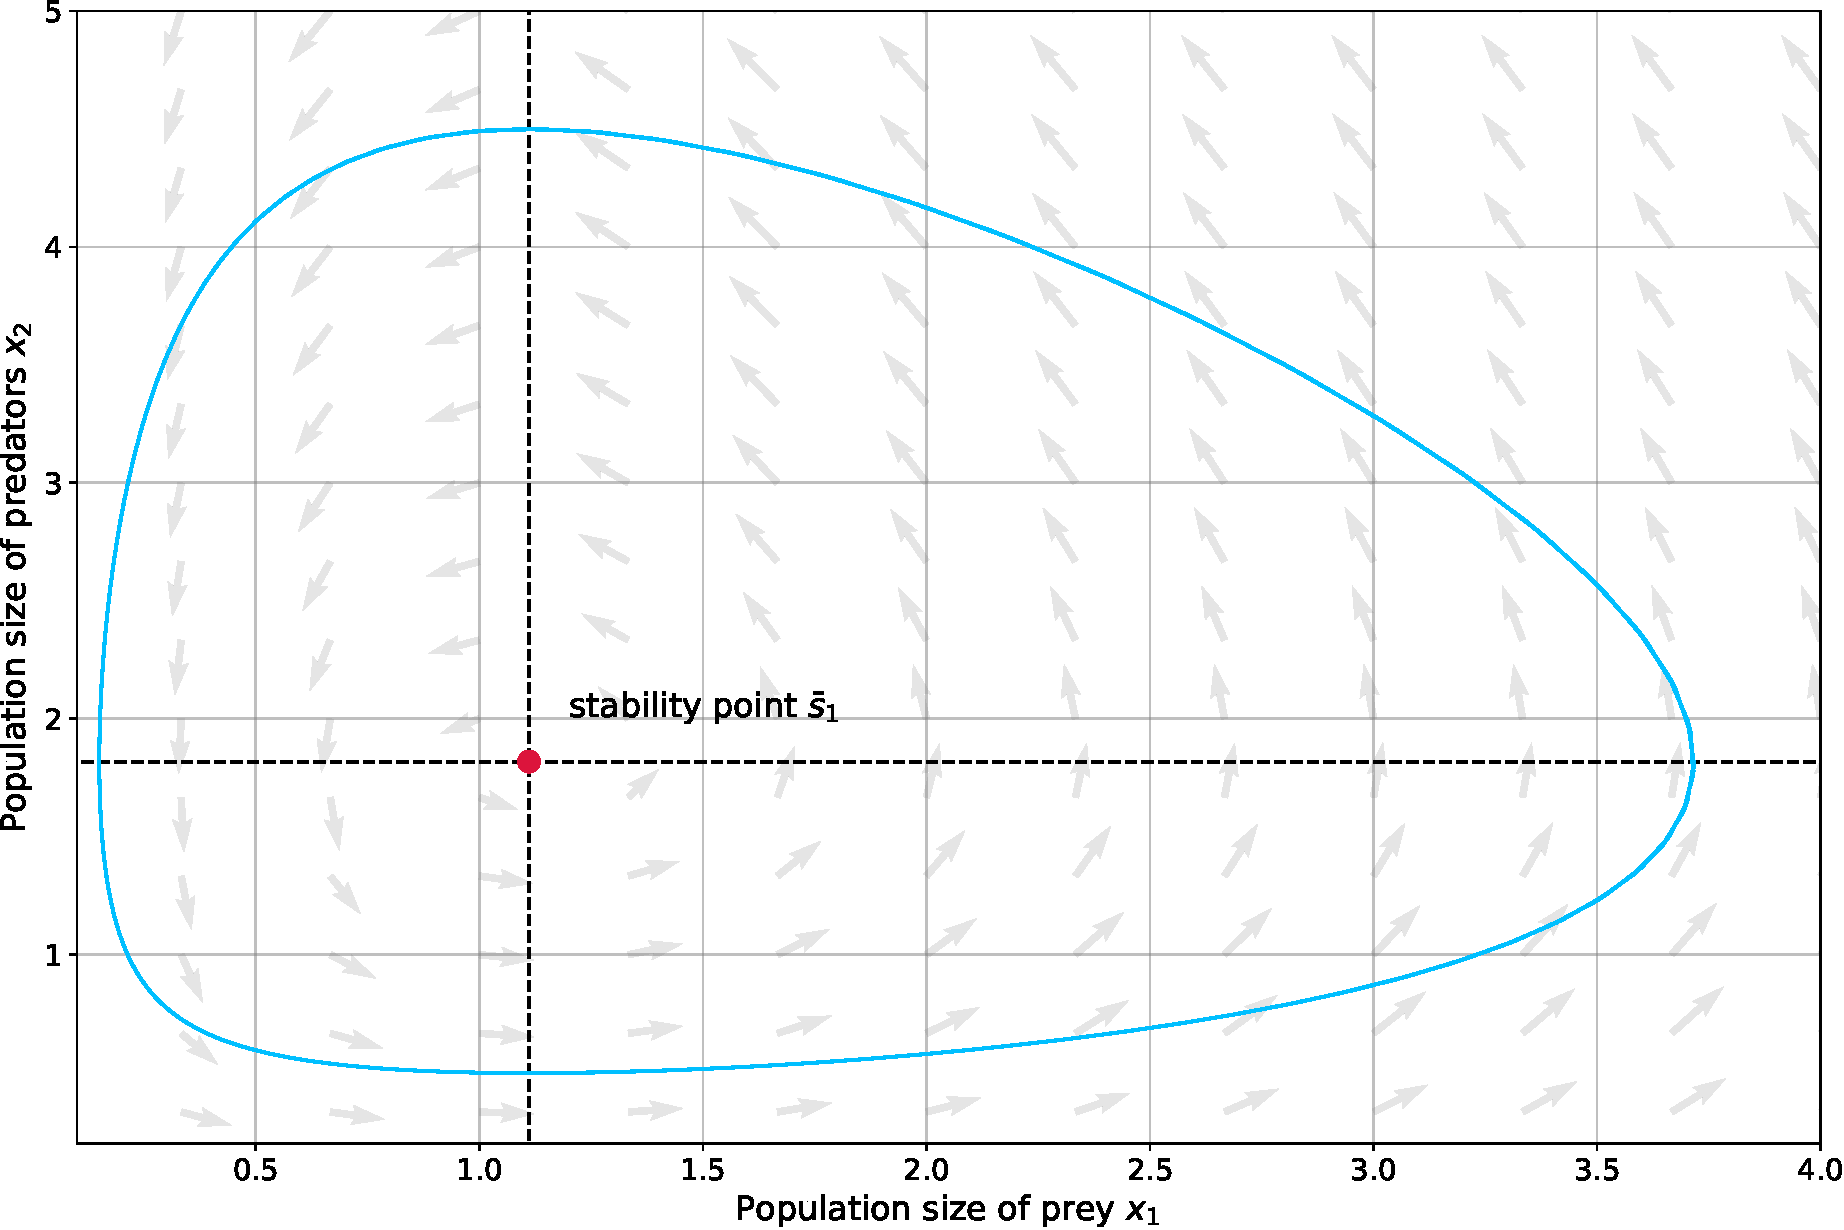
\includegraphics[width = \linewidth]{Grafiken/phase_plot_2d_simple_model.pdf}
        \caption{Slope field of system (\ref{eq:2d_simple_model}) and phase trajectory of the solution with initial value $x_1(0)= 1, x_2(0)=0.5$.}
        \label{fig:phase_plot_2d_simple_model}
    \end{figure}
    
\end{frame}
\subsubsection[Theoretical Results]{Theoretical Results}
\begin{frame}{Mathematical Properties}
\pnote{$\Bar{s}_0$ is unstable saddle point by linearization (Theorem of Hartman-Grobman)}
\pnote{$\Bar{s}_1$ is stable center by Lyapunov’s method}
\pnote{phase shift: explains phase shift in hare/lynx population dynamics}
\pnote{population mean: independent of intial values -> paradox of pesticide (shifting initial value)}

\only<1-2>{
\begin{remark}[Stability]

The 2-species predator-prey model has the fixed points
\begin{alignat*}{2}
        \Bar{s}_0 &= (0, 0)\ &&\mathrm{unstable\ saddle\ point} \\
        \Bar{s}_1 &= \left(\frac{r_2}{a_{21}}, \frac{r_1}{a_{12}}\right)\ &&\mathrm{stable\ center}.
\end{alignat*}
    
\end{remark}}\pause

\only<2>{
\begin{remark}[Periodicity]

The linearized system implies periodic solutions around $\Bar{s}_1$ with natural frequency $\omega = \sqrt{r_1r_2}$ and phase shift $\varphi = \frac{\pi}{2}$ \cite[6 \psq, 14 \psq]{stability_2d_predator_prey_model, 10.25365/thesis.45530}.
    
\end{remark}}

\only<3>{
\begin{remark}[Population Mean] 

    The mean values of the population sizes are
    \begin{align*}
        \Bar{x}_1 &= \frac{1}{T} \int_{t_0}^{t_0 + T} x_1(t)\ \mathrm{d}t = \frac{r_2}{a_{21}} \\
        \Bar{x}_2 &= \frac{1}{T} \int_{t_0}^{t_0 + T} x_2(t)\ \mathrm{d}t = \frac{r_1}{a_{12}}
    \end{align*}
for $T = \frac{2 \pi}{\omega}$. Therefore the means are independent of the initial values $x_1(0)$ and $x_2(0)$ \cite[14 \psqq]{10.25365/thesis.45530}.    
\end{remark}}

\end{frame}
\subsubsection{Paradox of Pesticides}
\begin{frame}{Predator-Prey Model with external Forcing}
\pnote{Phenomen of resurgence of pest was described many times in experiments}
\pnote{Apple orchards: flying instect (pest)}
\pnote{Extension: by approximation of delta function, modeling the effect of the pesticide}

\begin{definition}[2-dimensional Predator-Pest Model]
    The system of equations
    \begin{align}\label{eq: 2d_pesticide_model}
    \begin{split}
        \frac{\mathrm{d}x_1}{\mathrm{d}t} &= x_1 (r_1 - a_{12}x_2) - \alpha \laplace{(t-T)} \\
        \frac{\mathrm{d}x_2}{\mathrm{d}t} &= x_2 (-r_2 + a_{21}x_2) - \beta \laplace{(t-T)}
    \end{split}
    \end{align}
    for $r_1, r_2, a_{12}, a_{21}, \alpha, \beta > 0$ and
    \begin{align*}
     \laplace{(t-T)} = \left\{\begin{array}{ll} \frac{1}{\epsilon}, & t\in [T, T + \epsilon] \\
         0, & \mathrm{otherwise}\end{array}\right.
    \end{align*}
    is called predator-pest model \cite[2 \psqq]{pesticide_paradox}.
\end{definition}

\end{frame}
\begin{frame}{Pest Simulations}

\only<1>{
\begin{figure}
    \centering
    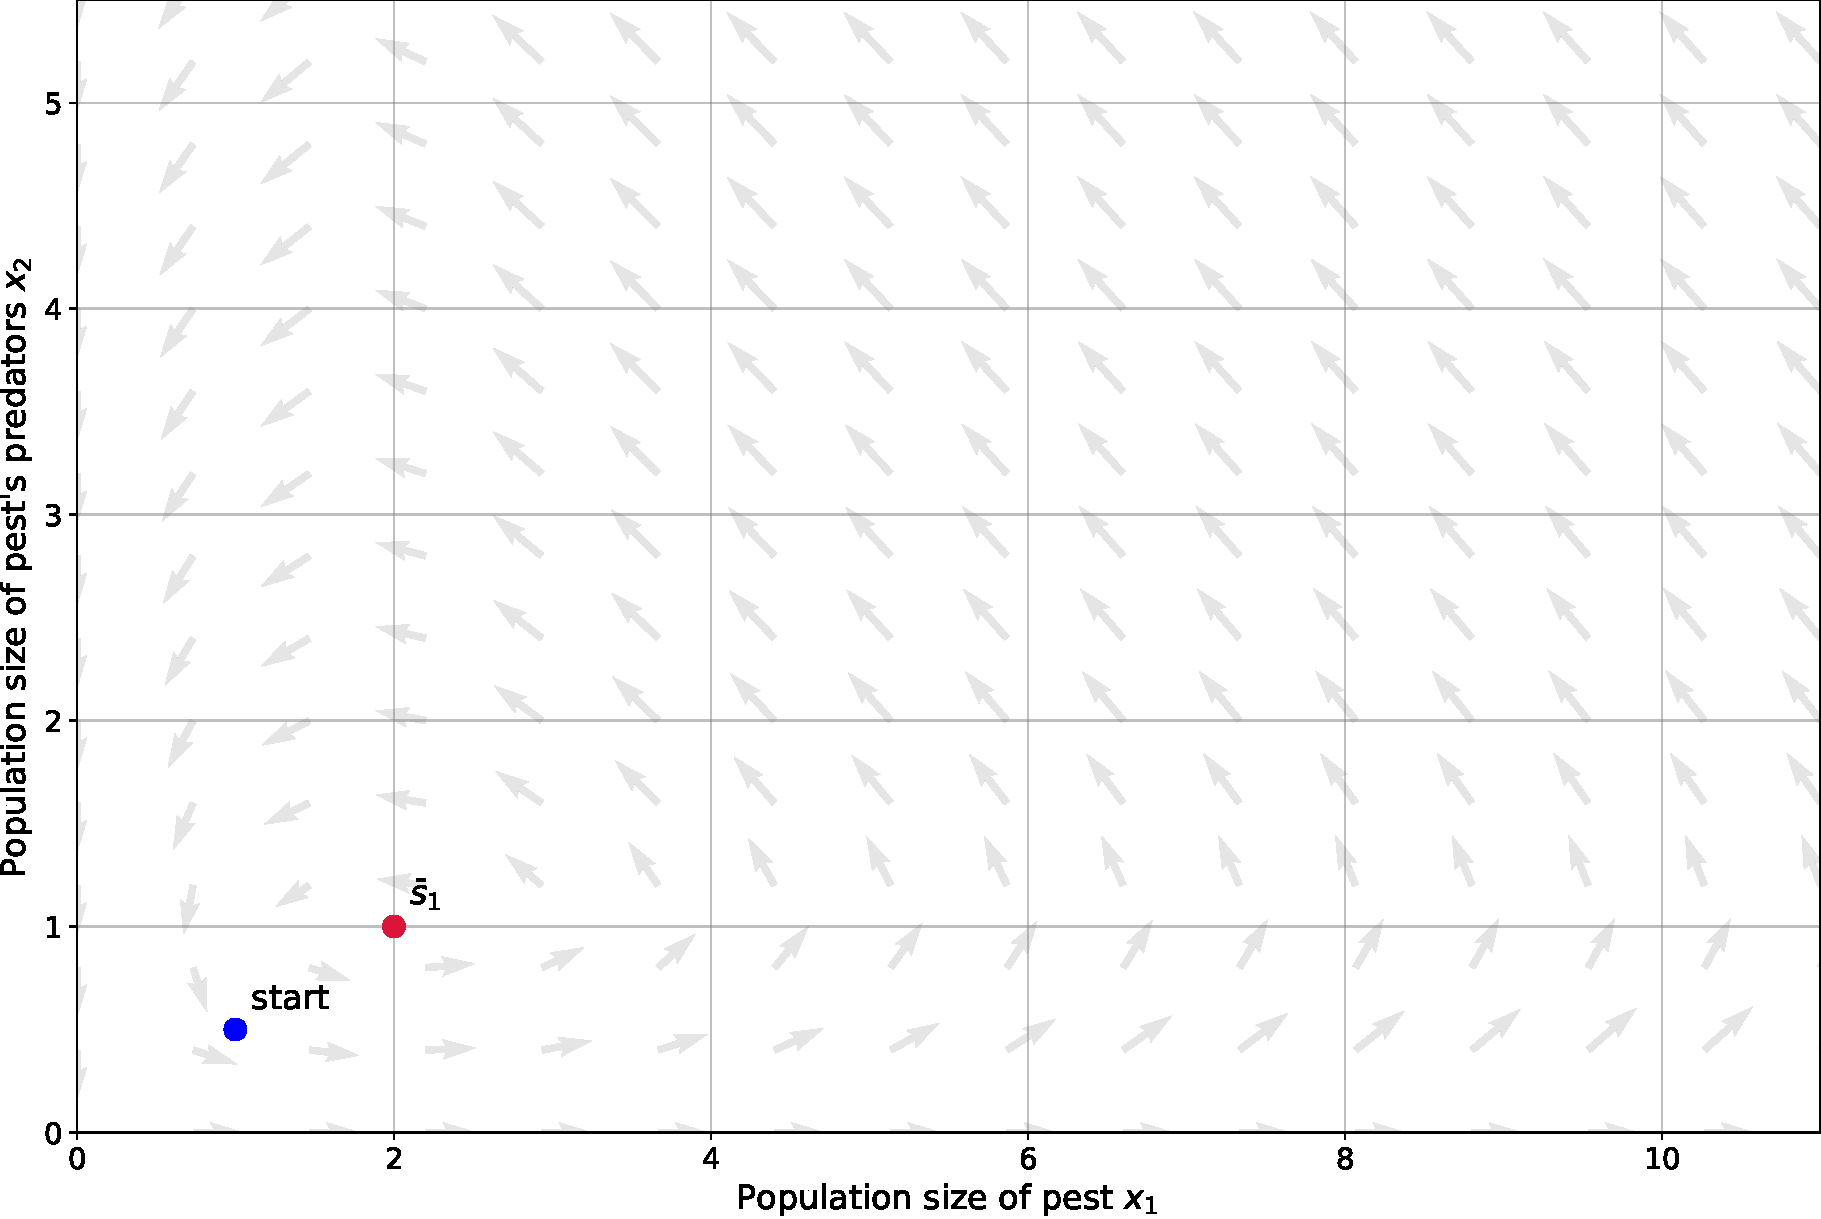
\includegraphics[width = \linewidth]{Grafiken/phase_plot_2d_pest_model_1.pdf}
    \caption{Trajectories of pesticide forced orbits in the 2-dimensional predator-pest-Model for different application times.}
    \label{fig:phase_plot_2d_pest_model_1}
\end{figure}}

\only<2>{
\begin{figure}
    \centering
    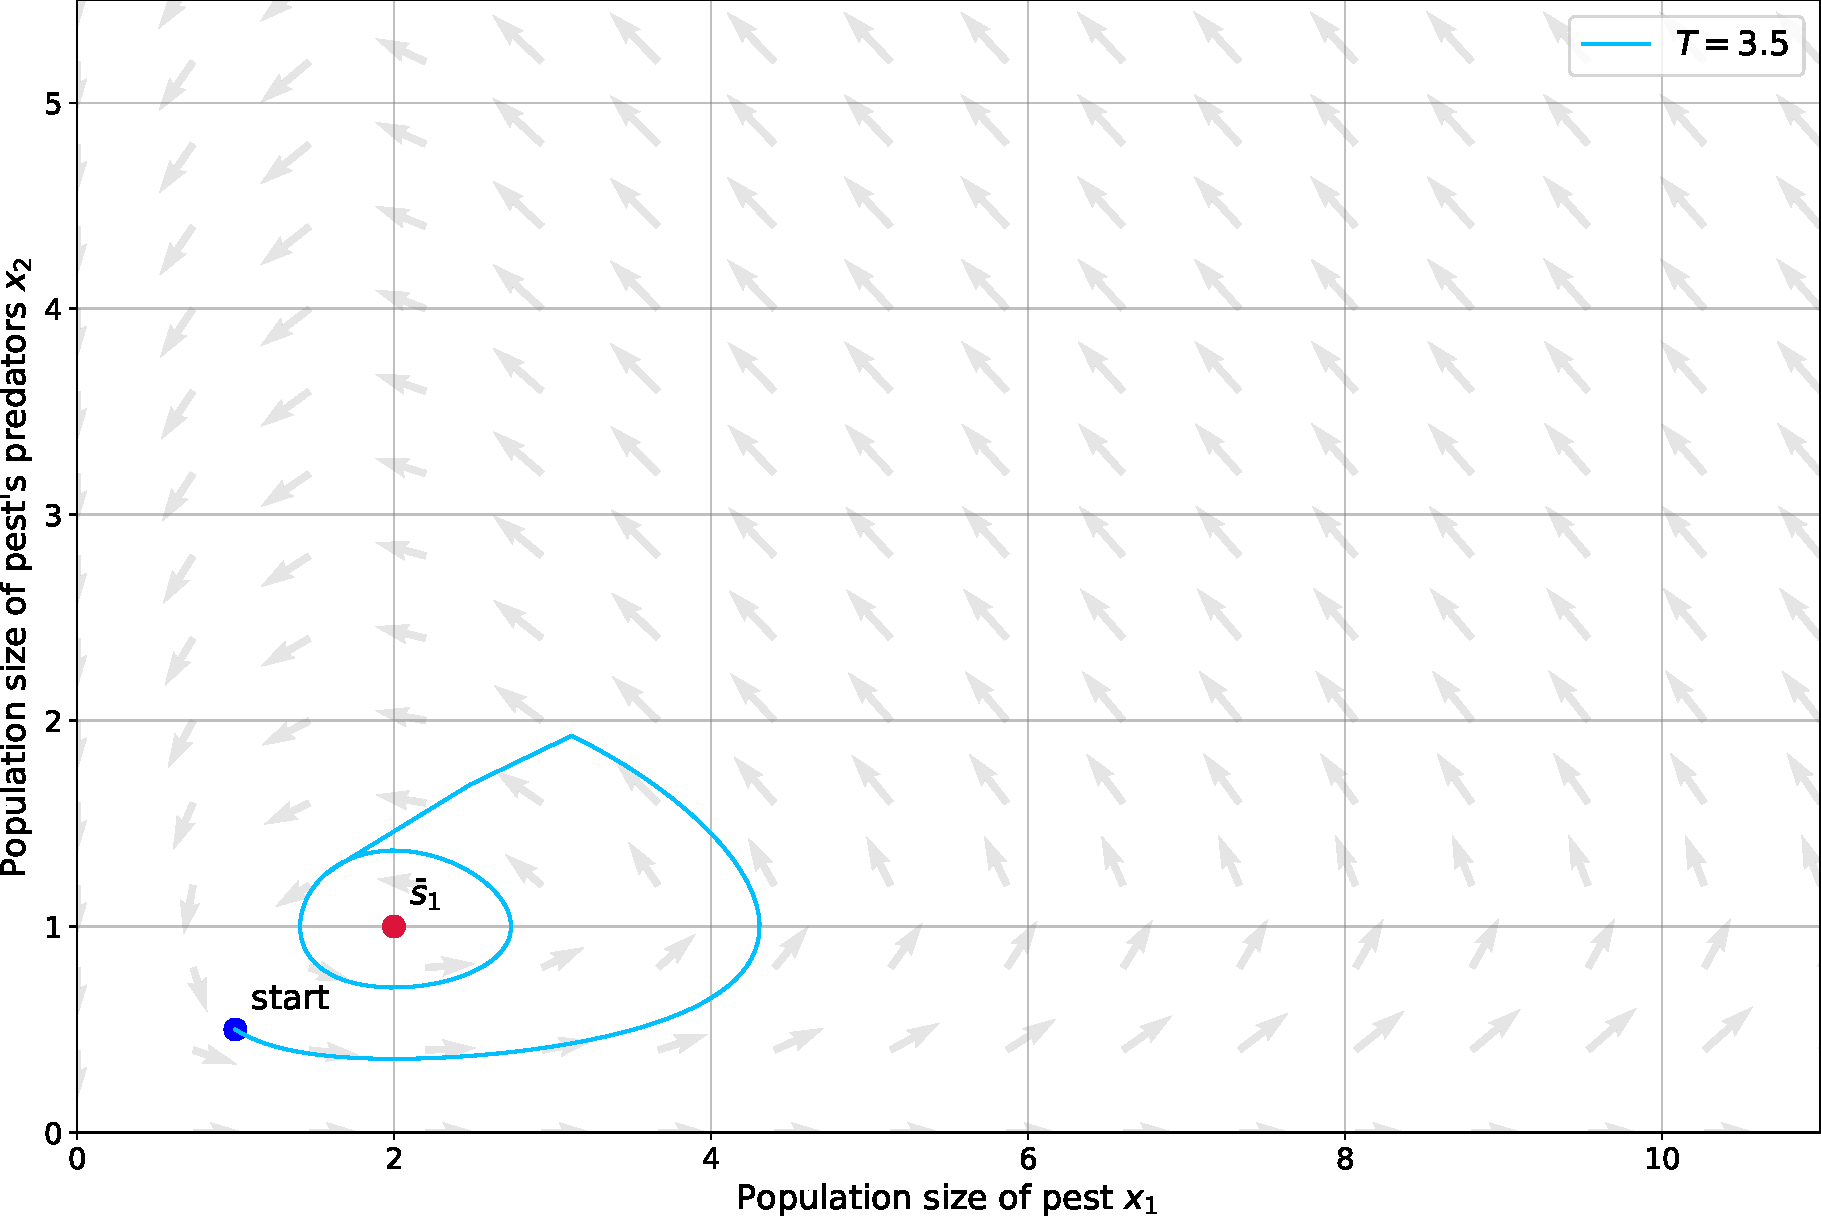
\includegraphics[width = \linewidth]{Grafiken/phase_plot_2d_pest_model_2.pdf}
    \caption{Trajectories of pesticide forced orbits in the 2-dimensional predator-pest-Model for different application times.}
    \label{fig:phase_plot_2d_pest_model_2}
\end{figure}}

\only<3>{
\begin{figure}
    \centering
    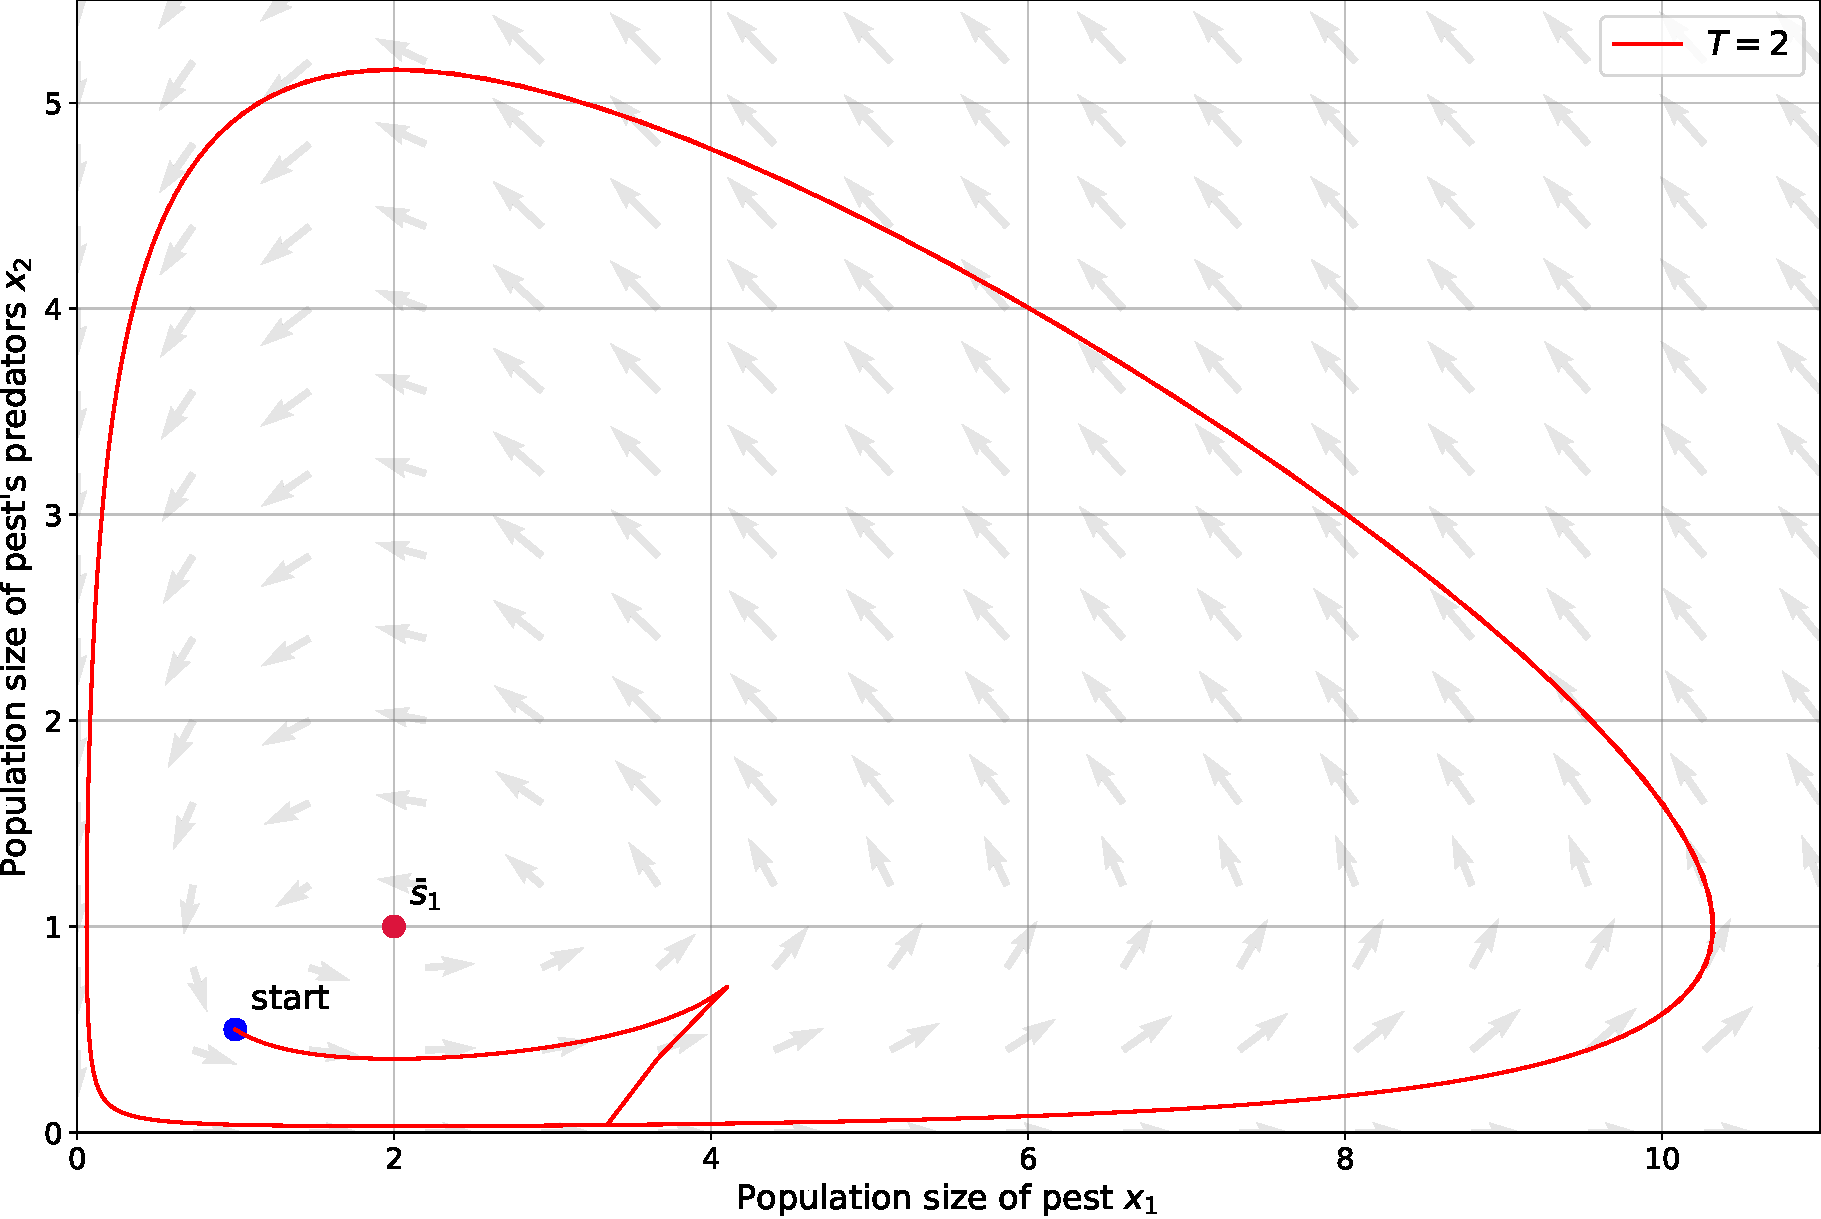
\includegraphics[width = \linewidth]{Grafiken/phase_plot_2d_pest_model_3.pdf}
    \caption{Trajectories of pesticide forced orbits in the 2-dimensional predator-pest-Model for different application times.}
    \label{fig:phase_plot_2d_pest_model_3}
\end{figure}}

\only<4>{
\begin{figure}
    \centering
    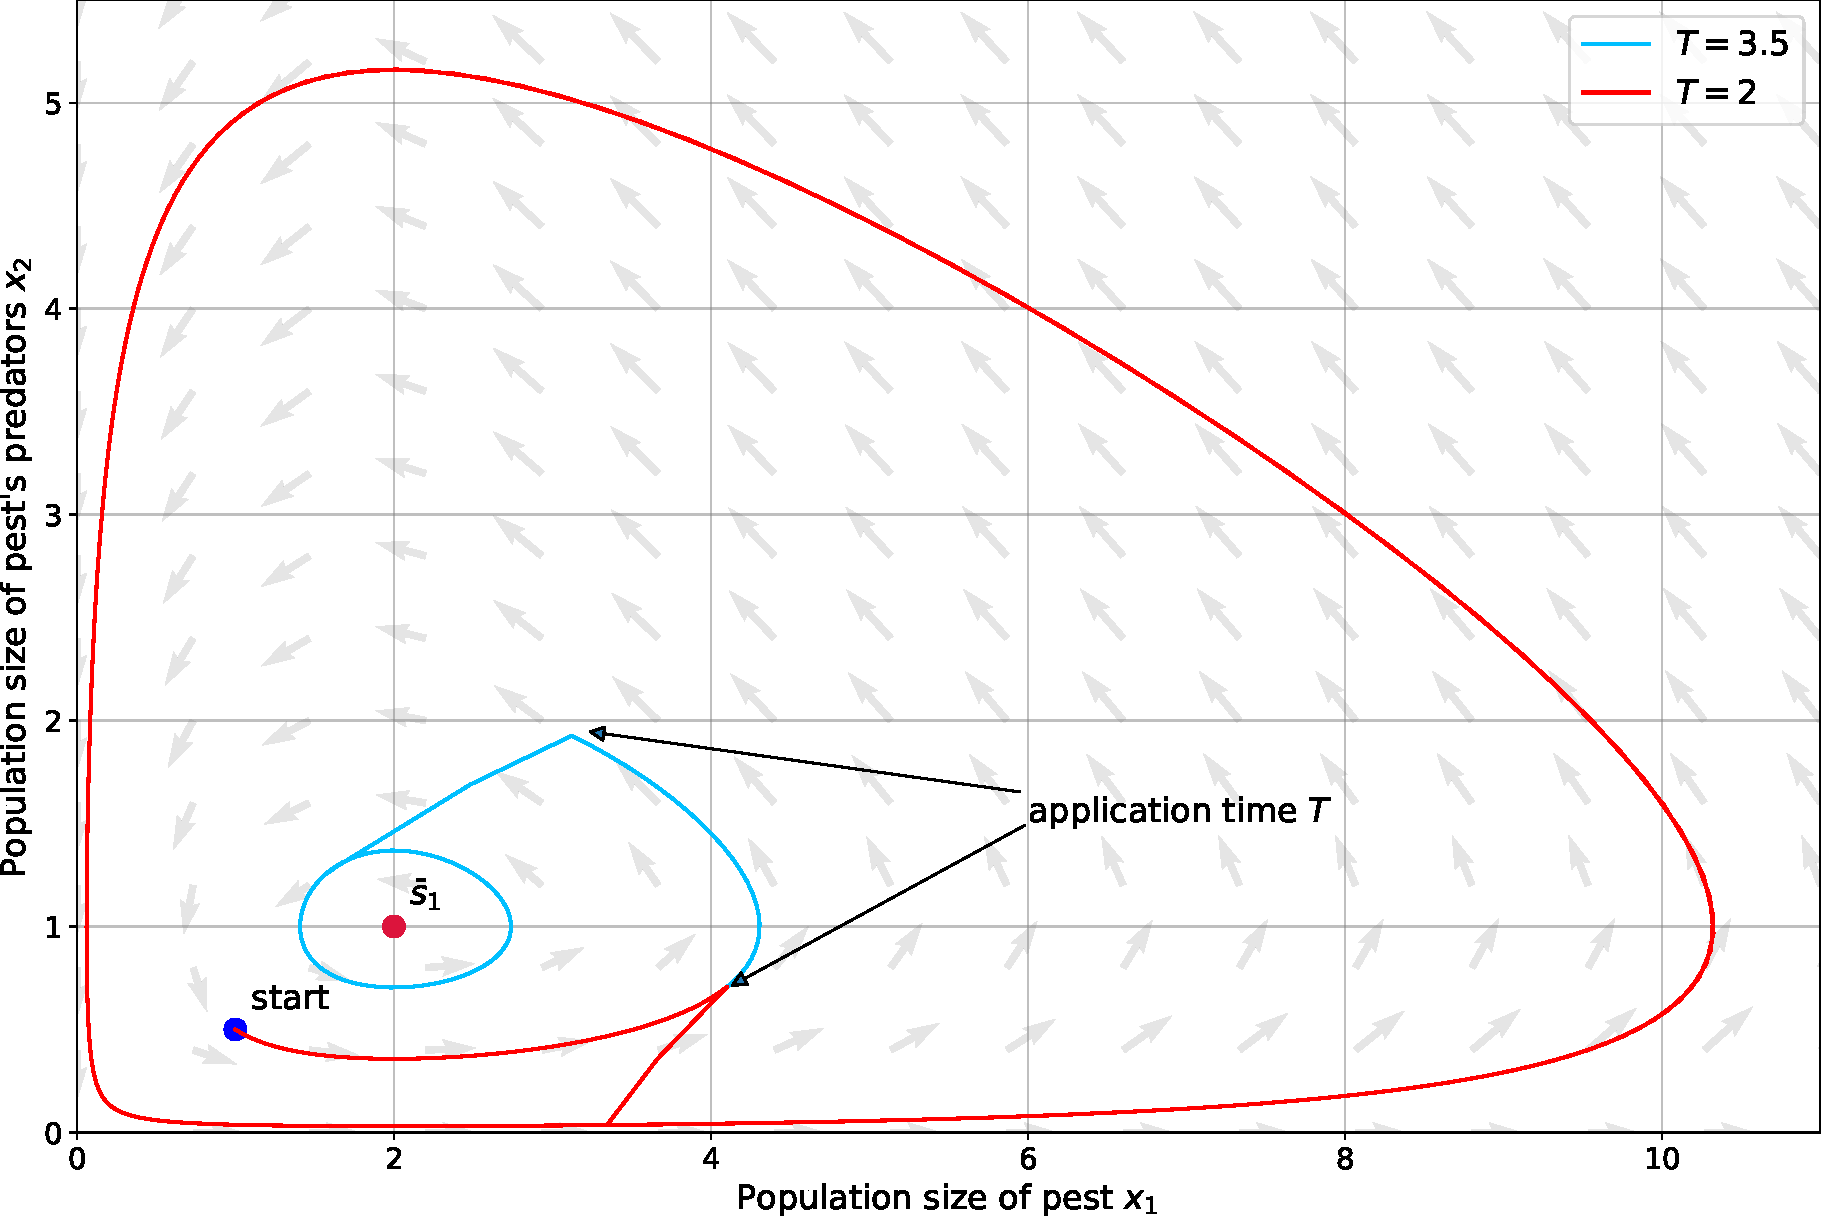
\includegraphics[width = \linewidth]{Grafiken/phase_plot_2d_pest_model_4.pdf}
    \caption{Trajectories of pesticide forced orbits in the 2-dimensional predator-pest model for different application times.}
    \label{fig:phase_plot_2d_pest_model_4}
\end{figure}}
    
\end{frame}
\subsection[Competitive System]{Competitive Lotka-Volterra Model}
\begin{frame}{Lotka-Volterra's Competition Model}
\pnote{adding intraspecific competition: rivalry for the same food source}
\pnote{limitation of the life sustaining resources}

\only<1>{
\begin{definition}[Competitive Lotka-Volterra Equations]
    The competitive Lotka-Volterra equations for a $n$-species model is the system
    \begin{align}\label{eq:competitive_lotka_volterra_equations}
        F_i(x) = \frac{\mathrm{d}x_i}{\mathrm{d}t} = x_i \left(r_i - \sum_{j = 1}^{n}a_{ij} x_j \right)
    \end{align}
    with $i = 1, 2, \ldots, n$ and $a_{ij}, r_i > 0$ for all $i, j = 1, 2, \ldots, n$ \cite[13]{stability_2d_predator_prey_model}.
\end{definition}}\pause
\refstepcounter{equation}

\only<2>{
\begin{remark}[Logistic Growth]
    The restriction to the $i$-th equation in system (\ref{eq:competitive_lotka_volterra_equations}) gives
    \begin{align*}
        \frac{\mathrm{d}x_i}{\mathrm{d}t} = x_i(r_i - a_{ii}x_i)
        =x_i r_i\left(1 - \frac{x_i}{K_i}\right)
    \end{align*}
    with $K_i = \frac{r_i}{a_{ii}}$, which is called the $i$-th carrying capacity \cite[197 \psqq]{theoryvsempiry}.
\end{remark}}
    
\end{frame}

\begin{frame}{Implications for the Ecosystem}

\begin{itemize}
    \item The life sustaining resources are limited.\pause
    \item The intraspecific competition between members of the $i$-th species hinders the growth of their population.\pause
    \item The interspecific competition leads to rivalry between the $n$ species.\pause
    \item The biotope is completely isolated from external influences \cite[265 \psqq, 202\psqq]{Volterra1931, theoryvsempiry}.
\end{itemize}
    
\end{frame}
\subsubsection{Simulations}
\begin{frame}{Numerical Results}
\pnote{Bistability: no stable point in the interior}

\begin{figure}
    \centering
    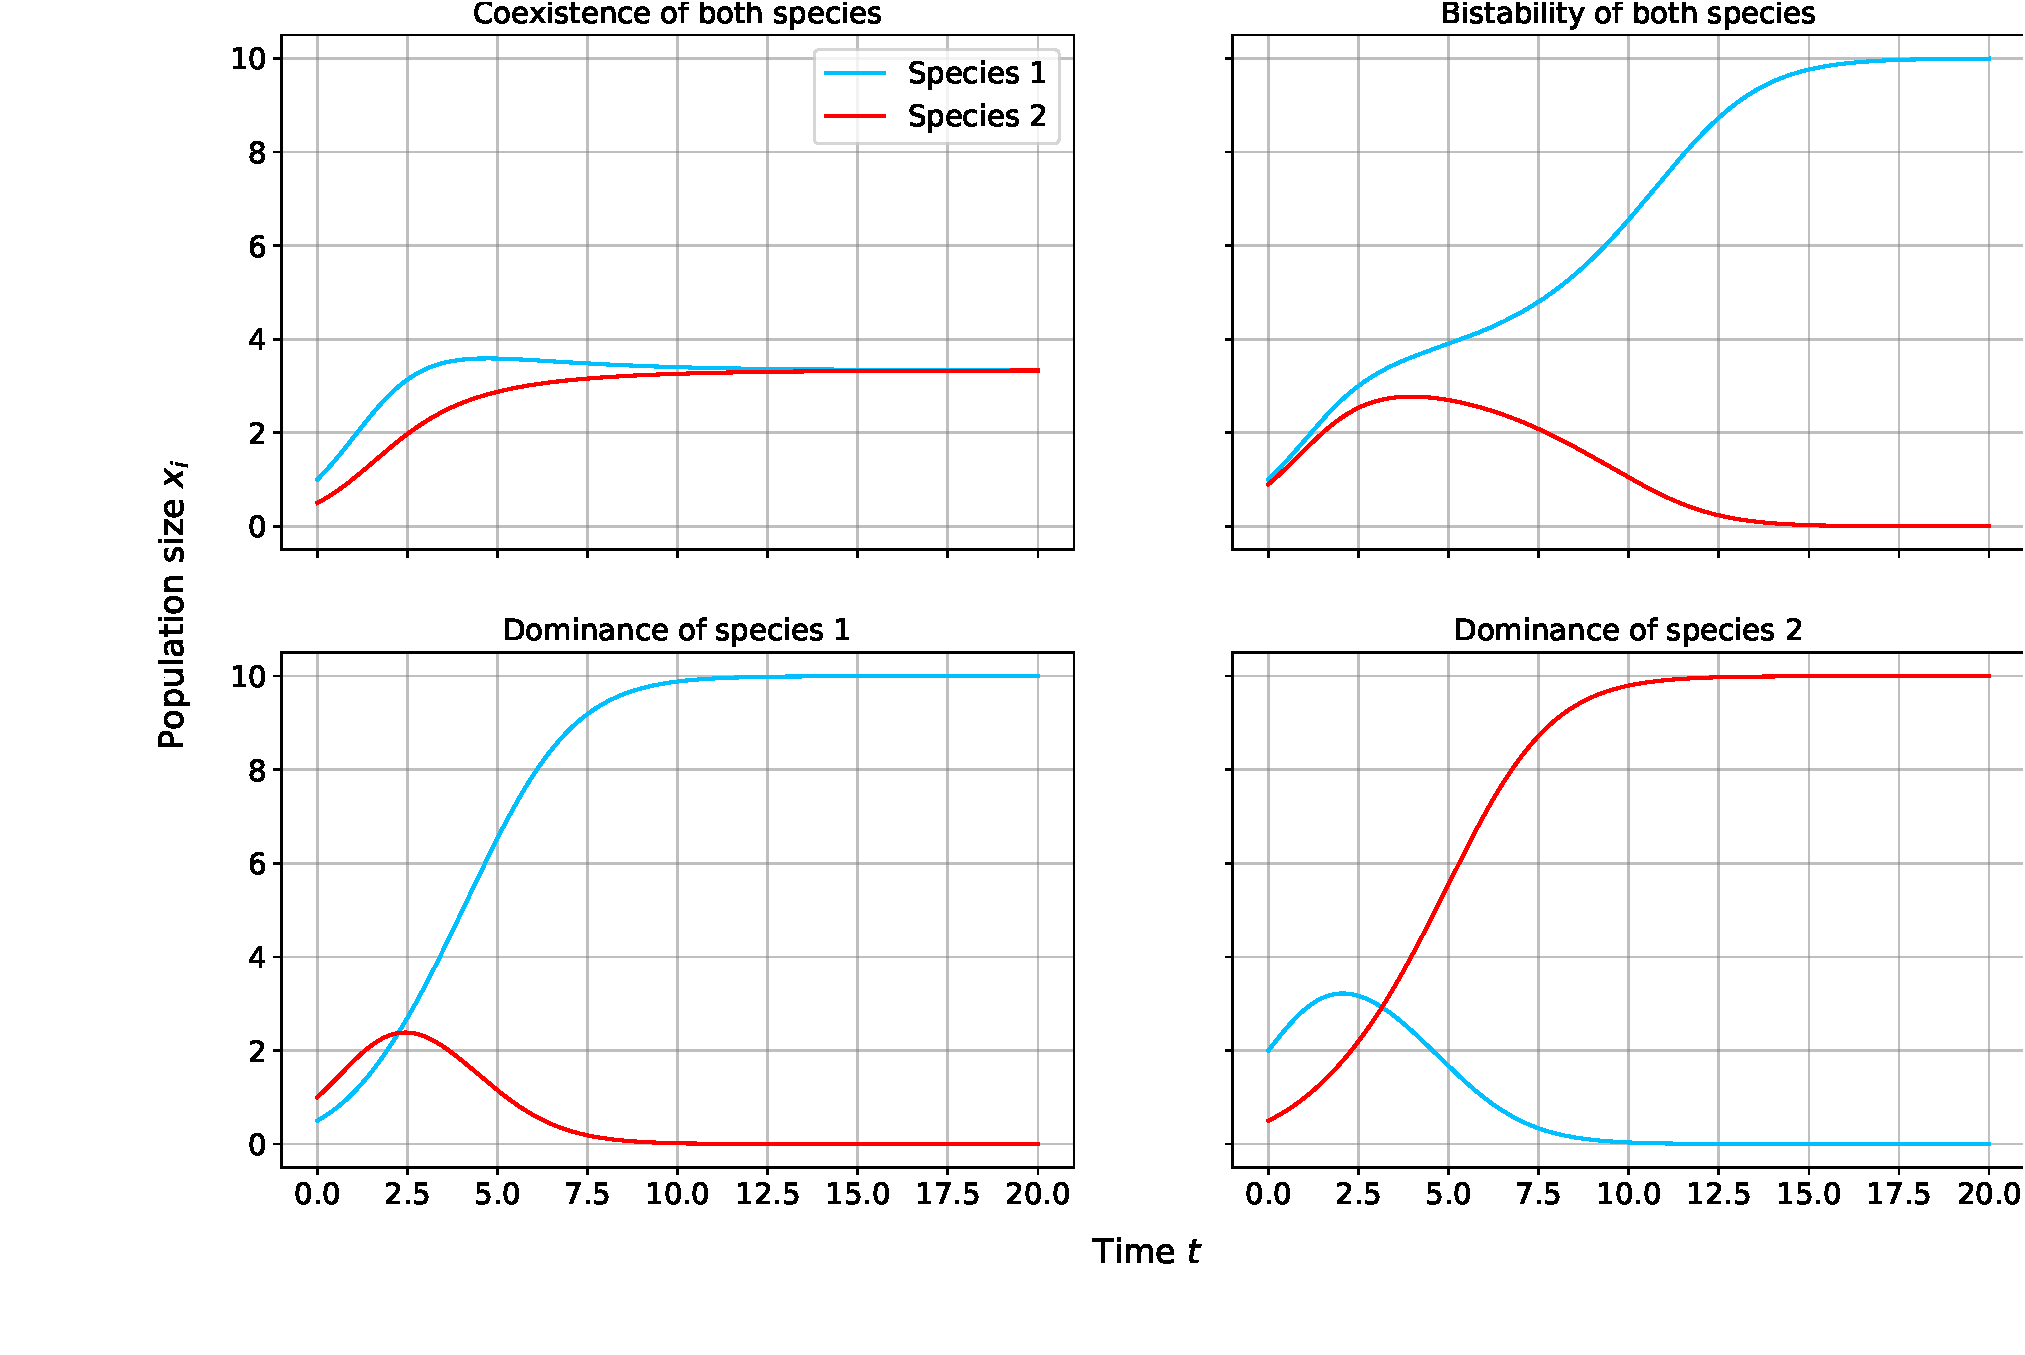
\includegraphics[width = \linewidth]{Grafiken/solution_2d_competitive_model.pdf}
    \caption{Classification of the 2-dimensional Lotka-Volterra competition model.}
    \label{fig:solution_2d_competitive_model}
\end{figure}
    
\end{frame}
\begin{frame}{Slope Field and Phase Space Representation}
\pnote{Classification: linearization (Hartman-Grobman Theorem)}

\begin{figure}
    \centering
    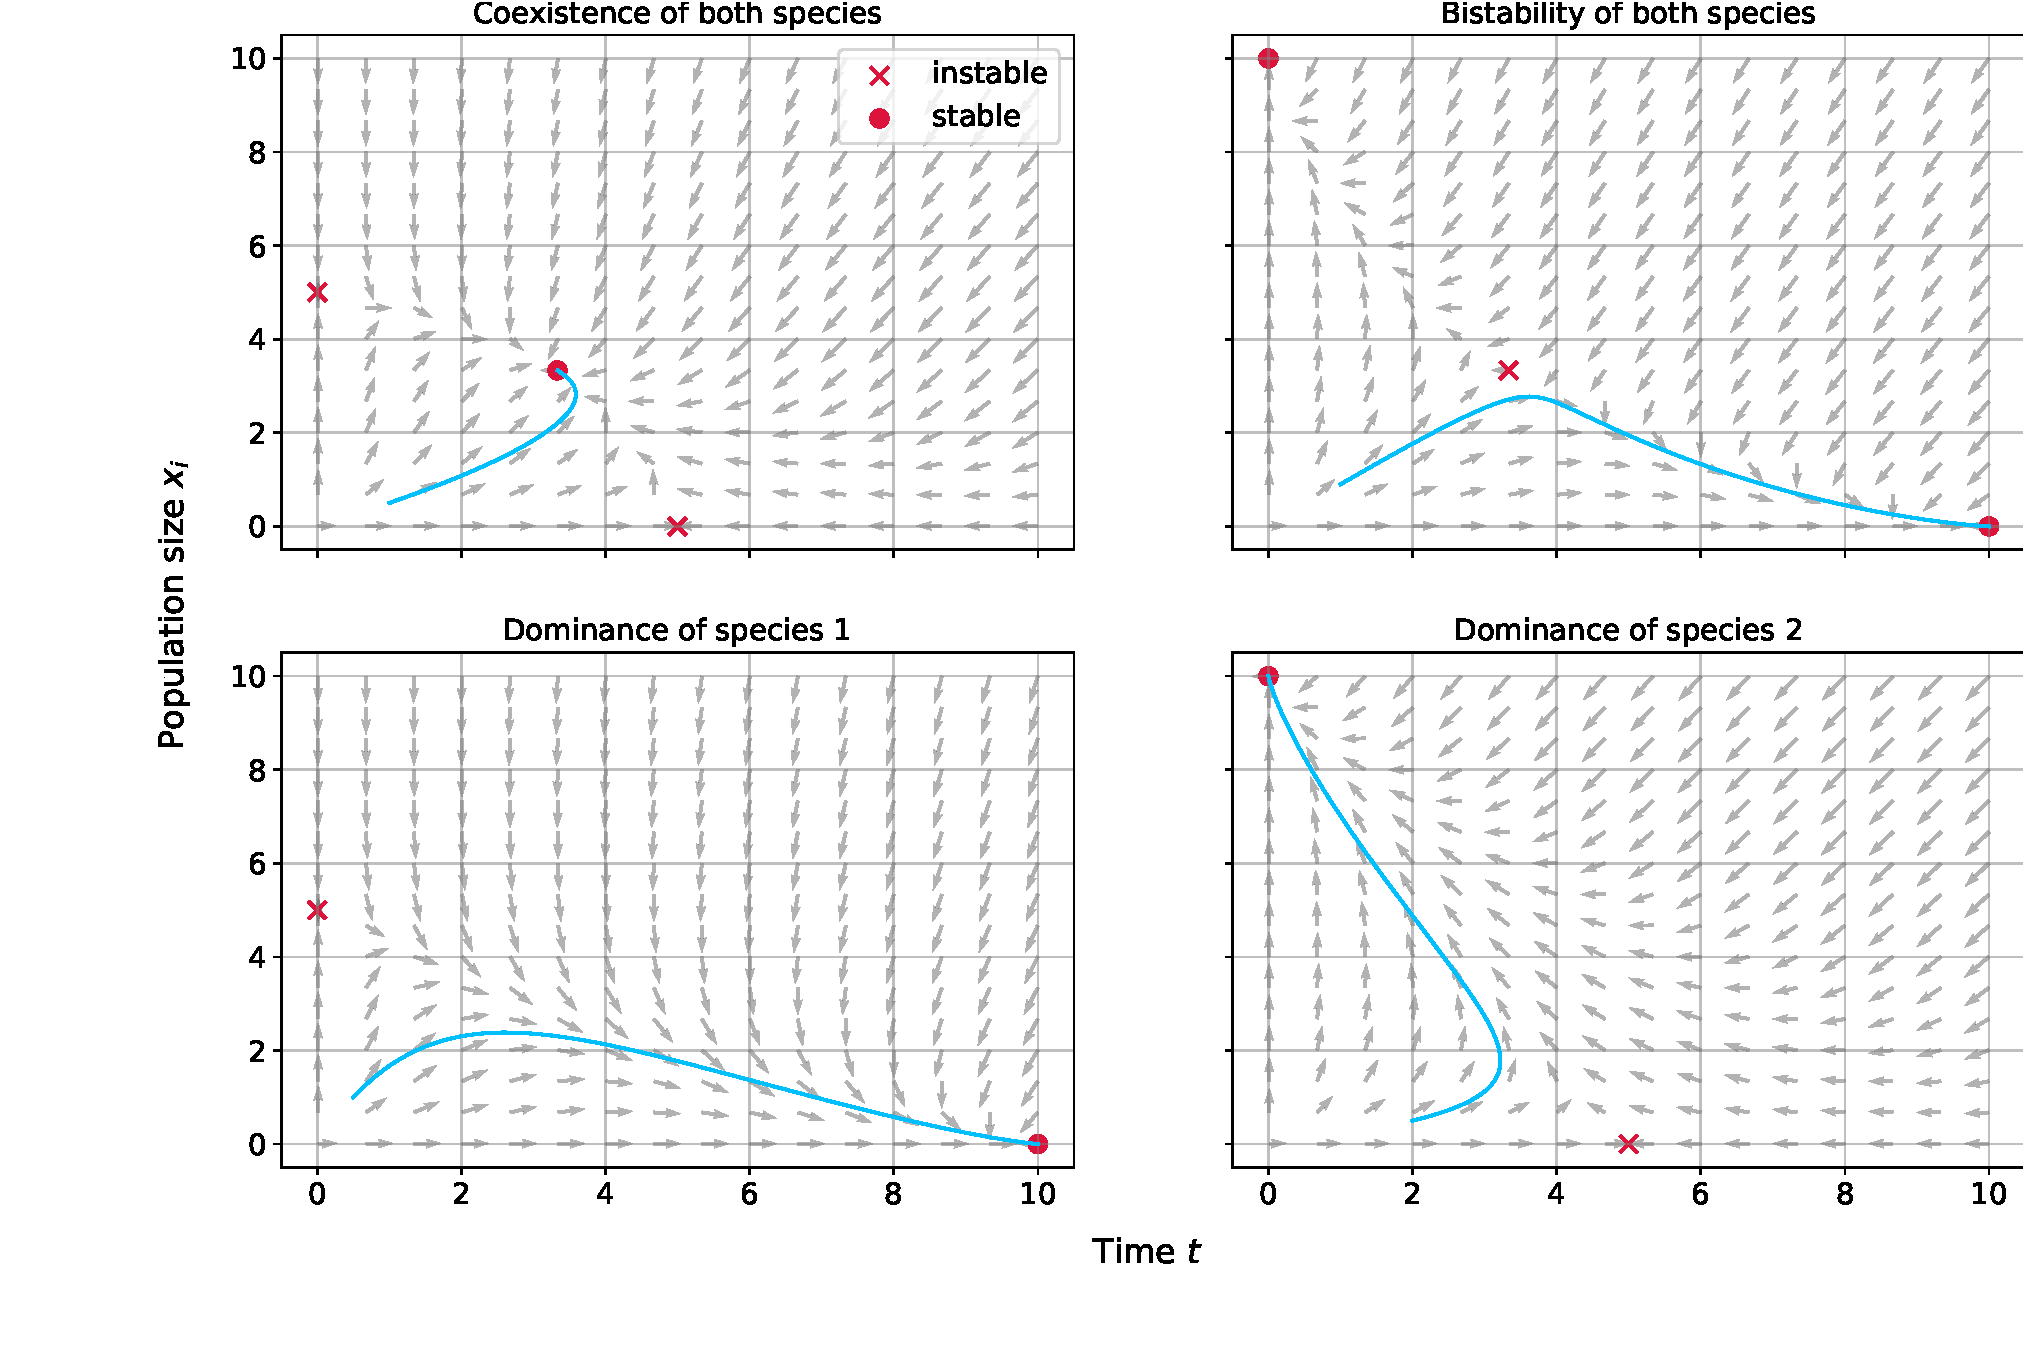
\includegraphics[width = \linewidth]{Grafiken/phase_plots_2d_competitive_model.pdf}
    \caption{Phase-space representation of the solutions of the 2-dimensional competition model.}
    \label{fig:phase_plots_2d_competitive_model}
\end{figure}
    
\end{frame}
\subsubsection{Gause's Law (CEP)}
\begin{frame}{Competitive Exclusion Principle}
\pnote{obeserved in parasitic fungi, paramecium, birds}
\pnote{not fully explained: biodiversity}
\pnote{Problems: lack of spatial component, competition-colonization trade off, adaptive radiation (darwin's finches)}


\begin{definition}[Gause's Law (1934)]
    Two species or populations cannot inhabit the same niche: one will consistently out-compete the other \cite[1 \psq, 2 \psq]{gauses_law, gauses_law2}.
\end{definition}

\begin{figure}
    \centering
    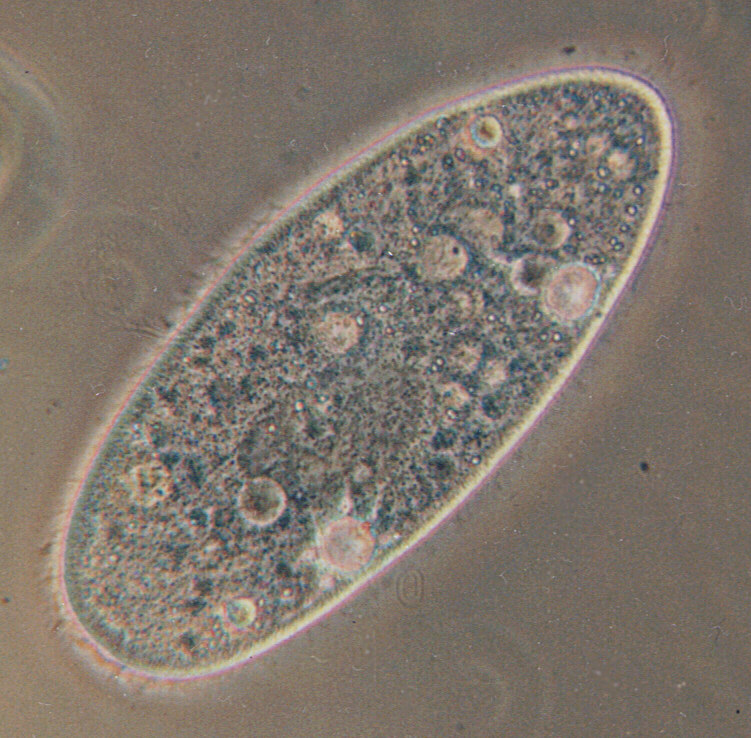
\includegraphics[width = 0.5\linewidth]{Grafiken/Paramecium.jpg}
    \caption{Image of paramecium aurelia.}
    \label{fig:paramecium}
\end{figure}
    
\end{frame}

\section{Extended Models}
\subsection{Seasonal Variation}
\begin{frame}{Seasonal Effects}

\begin{remark}[Lotka-Volterra Model with seasonal Fluctuations]
        The Lotka-Volterra equations for a $n$-species model with seasonal term reads
    \begin{align}\label{eq:lotka_volterra_with_seasons}
        F_i(x) = \frac{\mathrm{d}x_i}{\mathrm{d}t} = x_i \left(r_i + \mu_i \sin(\nu t) + \sum_{j = 1}^{n}a_{ij} x_j \right)
    \end{align}
    with $i = 1, 2, \ldots, n$. The parameter $\mu_i$ represents the impact of the environmental change for the $i$-th species \cite[7 \psq]{predatorpreymodel}.
\end{remark}
    
\end{frame}
\subsection{Delay Kernels}
\begin{frame}{Delayed Interaction Effects}

\begin{remark}[Lotka-Volterra Model with Delay Kernels]
        The Lotka-Volterra equations for a $n$-species model with changing rate of interaction is the system
    \begin{align}\label{eq:lotka_volterra_with_delay}
        F_i(x) = \frac{\mathrm{d}x_i}{\mathrm{d}t} = x_i \left(r_i + \sum_{j = 1}^{n} \int_{-\infty}^{t}F_{ij}(t - \tau)x_j(\tau) \ \mathrm{d}\tau \right)
    \end{align}
    with $i = 1, 2, \ldots, n$. The functions $F_{ij}$ are non-negative continuous delay kernels representing the changing rate of interaction between species $i$ and $j$ with respect to the past \cite[8]{predatorpreymodel}.
\end{remark}
    
\end{frame}

\appendix
\begin{frame}[allowframebreaks]
\nocite{*}
\printbibliography
\end{frame}

\end{document}
